% !TeX program = lualatex
% !TeX encoding = utf8
\documentclass[aspectratio=169,10pt]{beamer}

\usetheme[progressbar=frametitle, numbering=fraction]{metropolis}

% Paleta de colores FIUBA
\definecolor{fiubaBlue}{RGB}{0, 75, 135}
\definecolor{fiubaLight}{RGB}{230, 240, 250}
\definecolor{accentGreen}{RGB}{46, 139, 87}
\definecolor{accentOrange}{RGB}{230, 126, 34}

\setbeamercolor{palette primary}{bg=fiubaBlue}
\setbeamercolor{progress bar}{fg=accentOrange, bg=fiubaBlue!20}
\setbeamercolor{alerted text}{fg=accentOrange}

\usepackage{fontspec}
\usepackage[spanish]{babel}
\usepackage{graphicx}
\usepackage{booktabs}
\usepackage{multicol}
\usepackage{tikz}
\usetikzlibrary{arrows.meta, positioning, shapes.geometric}

\graphicspath{{../paper/figures/}}

% Metadata
\title[Autocobro Despensa]{Detección de Productos en Tiempo Real\\para Autocobro en Despensa Comunitaria}
\subtitle{Visión por Computadora II --- CEIA FIUBA}
\author[Grupo 4]{María Belén Cattaneo \and Nicolás Valentín Ciarrapico \and Sabrina Daiana Pryszczuk}
\institute[CEIA FIUBA]{CEIA --- Facultad de Ingeniería --- Universidad de Buenos Aires}
\date{Abril 2026}

\begin{document}

% ============================================================
% SLIDE 1: Título
% ============================================================
\begin{frame}[plain]
  \maketitle
\end{frame}

% ============================================================
% SLIDE 2: El Problema
% ============================================================
\begin{frame}{El Problema}
  \begin{columns}[T]
    \begin{column}{0.55\textwidth}
      \begin{block}{Contexto}
        Una \textbf{mutual} gestiona una despensa comunitaria con $\sim$60 productos.
      \end{block}
      \vspace{0.3cm}
      \begin{itemize}
        \item El proceso de checkout es \textbf{manual} y lento
        \item Soluciones comerciales (Amazon Go) cuestan \textbf{millones de USD}
        \item Se necesita un sistema \textbf{accesible} para organizaciones pequeñas
      \end{itemize}
    \end{column}
    \begin{column}{0.4\textwidth}
      \begin{block}{Nuestra propuesta}
        Sistema de autocobro basado \textbf{exclusivamente en visión por computadora}, de bajo costo (\textbf{140--190 USD}).
      \end{block}
    \end{column}
  \end{columns}
\end{frame}

% ============================================================
% SLIDE 3: Solución Propuesta + Arquitectura
% ============================================================
\begin{frame}{Solución Propuesta}
  \begin{columns}[T]
    \begin{column}{0.45\textwidth}
      \begin{enumerate}
        \item Cámara cenital sobre mesa de control
        \item El asociado coloca productos de a uno
        \item El sistema detecta y clasifica en tiempo real
        \item Se genera la lista de compra automáticamente
      \end{enumerate}
      \vspace{0.3cm}
      \begin{block}{Hardware}
        Raspberry Pi 5 + webcam USB + monitor HDMI
      \end{block}
    \end{column}
    \begin{column}{0.5\textwidth}
      \centering
      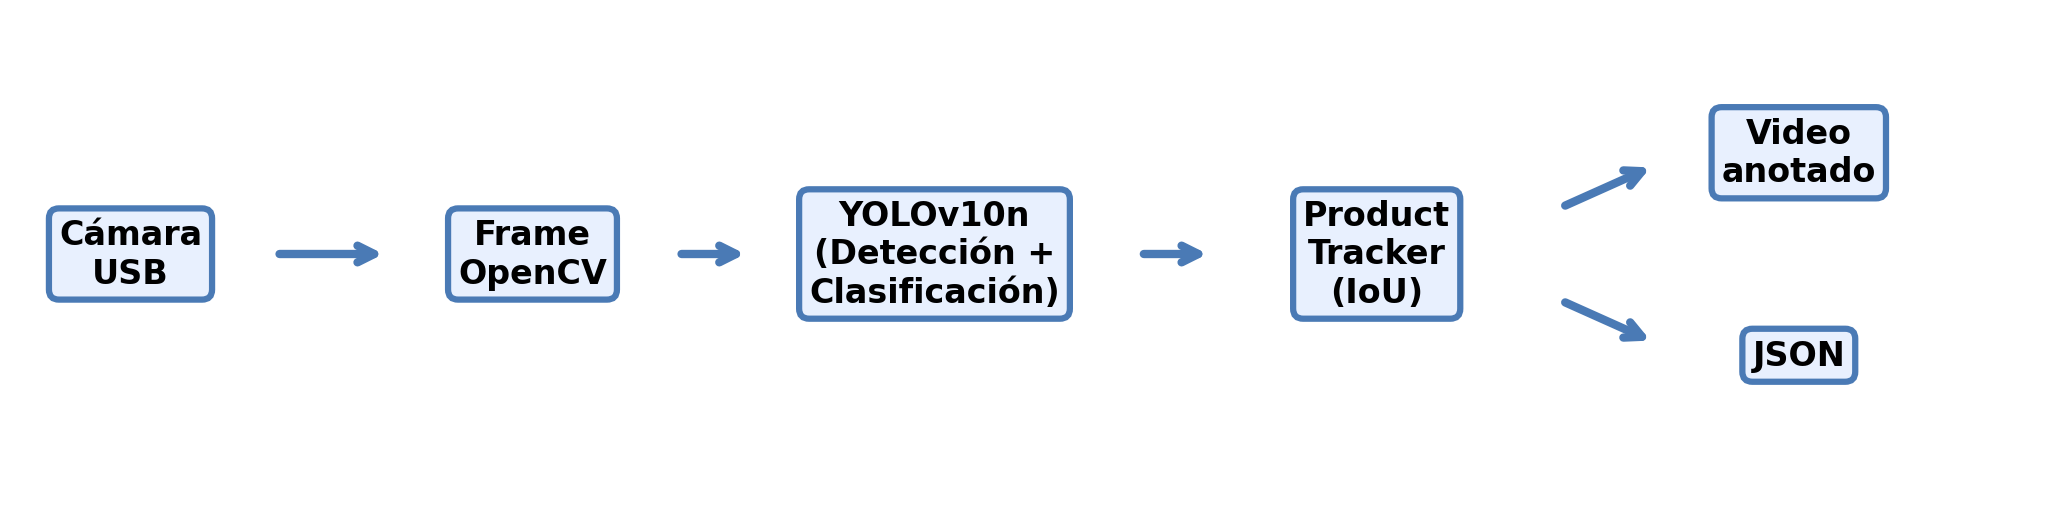
\includegraphics[width=\linewidth]{arquitectura.png}
    \end{column}
  \end{columns}
\end{frame}

% ============================================================
% SLIDE 4: Dataset
% ============================================================
\begin{frame}{Dataset Propio}
  \begin{columns}[T]
    \begin{column}{0.5\textwidth}
      \begin{block}{10 clases de productos}
        \small
        \begin{multicols}{2}
          \begin{enumerate}
            \item aceite 1L
            \item aceite 4L
            \item dulce de leche
            \item fideos
            \item leche descremada
            \item leche entera
            \item miel
            \item polenta
            \item tomate
            \item yerba
          \end{enumerate}
        \end{multicols}
      \end{block}
      \vspace{0.2cm}
      Incluye pares \textbf{visualmente similares}:\\
      leche descremada/entera, aceite 1L/4L
    \end{column}
    \begin{column}{0.45\textwidth}
      \begin{block}{Composición}
        \centering
        \begin{tabular}{lrr}
          \toprule
                     & \textbf{Individual} & \textbf{Multi} \\
          \midrule
          Train      & 102   & 132  \\
          Validation & 13    & 19   \\
          Test       & 12    & 18   \\
          \midrule
          \textbf{Total} & \textbf{127} & \textbf{169} \\
          \bottomrule
        \end{tabular}
      \end{block}
      \vspace{0.2cm}
      \small
      Captura cenital, 1080p, fondo uniforme.\\
      Anotado en \textbf{Roboflow} (formato YOLO).
    \end{column}
  \end{columns}
\end{frame}

% ============================================================
% SLIDE 5: Modelo y Entrenamiento
% ============================================================
\begin{frame}{Modelo y Entrenamiento}
  \begin{columns}[T]
    \begin{column}{0.5\textwidth}
      \begin{block}{¿Por qué YOLO?}
        \begin{itemize}
          \item \textbf{Single-stage:} detección + clasificación en un paso
          \item \textbf{Tiempo real:} $>$15 FPS
          \item \textbf{Variante nano:} 2.3M parámetros\\
                $\Rightarrow$ viable en Raspberry Pi 5
        \end{itemize}
      \end{block}
    \end{column}
    \begin{column}{0.45\textwidth}
      \begin{block}{Configuración}
        \centering
        \begin{tabular}{ll}
          \toprule
          Épocas        & 100 (early stop 20) \\
          Batch size    & 16 \\
          Imagen        & 640$\times$640 \\
          Optimizador   & SGD (lr=0.01) \\
          Transfer      & COCO pre-trained \\
          Hardware      & Intel i5-6200U \\
          \bottomrule
        \end{tabular}
      \end{block}
    \end{column}
  \end{columns}
  \vspace{0.3cm}
  \begin{block}{Data Augmentation (crítico)}
    Mosaic ($p$=1.0) + flip horizontal ($p$=0.5) + jitter HSV.
    Sin augmentation: mAP@0.5 cae de 0.833 a \alert{0.512} en test.
  \end{block}
\end{frame}

% ============================================================
% SLIDE 6: Benchmark de Arquitecturas
% ============================================================
\begin{frame}{Benchmark de Arquitecturas Nano}
  \centering
  \begin{table}
    \begin{tabular}{lcccc}
      \toprule
      \textbf{Modelo} & \textbf{Parámetros} & \textbf{Inferencia} & \textbf{mAP@0.5} & \textbf{mAP@0.5:0.95} \\
      \midrule
      YOLOv8n  & 3.0 M            & 246.2 ms         & \textbf{0.967} & 0.835 \\
      YOLOv10n & \textbf{2.2 M}   & 213.0 ms         & 0.813          & 0.774 \\
      YOLO11n  & 2.5 M            & \textbf{205.7 ms} & \textbf{0.967} & \textbf{0.889} \\
      \midrule
      RT-DETR-L & --- & --- & \multicolumn{2}{c}{\textit{Segfault (sin memoria)}} \\
      \bottomrule
    \end{tabular}
  \end{table}
  \vspace{0.3cm}
  \begin{block}{Conclusión}
    \textbf{YOLO11n} seleccionado: mejor mAP@0.5:0.95 (\textbf{0.889}), mayor velocidad (\textbf{205.7 ms/img}), y empata en mAP@0.5 con YOLOv8n.
  \end{block}
\end{frame}

% ============================================================
% SLIDE 7: Pipeline de Inferencia
% ============================================================
\begin{frame}{Pipeline de Inferencia}
  \begin{block}{Lógica de registro multi-frame}
    \centering
    \begin{tikzpicture}[
      node distance=1cm and 1.2cm,
      every node/.style={font=\small},
      block/.style={rectangle, draw=fiubaBlue, fill=fiubaLight, rounded corners, minimum height=0.9cm, minimum width=2cm, align=center, thick},
      arrow/.style={-{Stealth[length=3mm]}, thick, fiubaBlue}
    ]
      \node[block] (det) {Detección\\YOLO11n};
      \node[block, right=of det] (iou) {Matching\\IoU $\geq$ 0.3};
      \node[block, right=of iou] (conf) {Confirmación\\$\geq$5 frames\\conf $\geq$ 0.5};
      \node[block, right=of conf] (reg) {Registro\\estable};

      \draw[arrow] (det) -- (iou);
      \draw[arrow] (iou) -- (conf);
      \draw[arrow] (conf) -- (reg);
    \end{tikzpicture}
  \end{block}
  \vspace{0.3cm}
  \begin{columns}[T]
    \begin{column}{0.48\textwidth}
      \begin{itemize}
        \item \textcolor{accentGreen}{\textbf{Verde:}} producto confirmado
        \item \textcolor{yellow!80!black}{\textbf{Amarillo:}} pendiente de confirmación
        \item \textcolor{accentOrange}{\textbf{Naranja:}} advertencia (baja confianza)
      \end{itemize}
    \end{column}
    \begin{column}{0.48\textwidth}
      \begin{itemize}
        \item Tolerancia de oclusión: 10 frames ($\sim$333 ms)
        \item Sin tracker complejo (productos estáticos)
        \item Salida: video anotado + JSON
      \end{itemize}
    \end{column}
  \end{columns}
\end{frame}

% ============================================================
% SLIDE 8: Resultados — Validación
% ============================================================
\begin{frame}{Resultados: Validación (YOLO11n)}
  \begin{columns}[T]
    \begin{column}{0.48\textwidth}
      \centering
      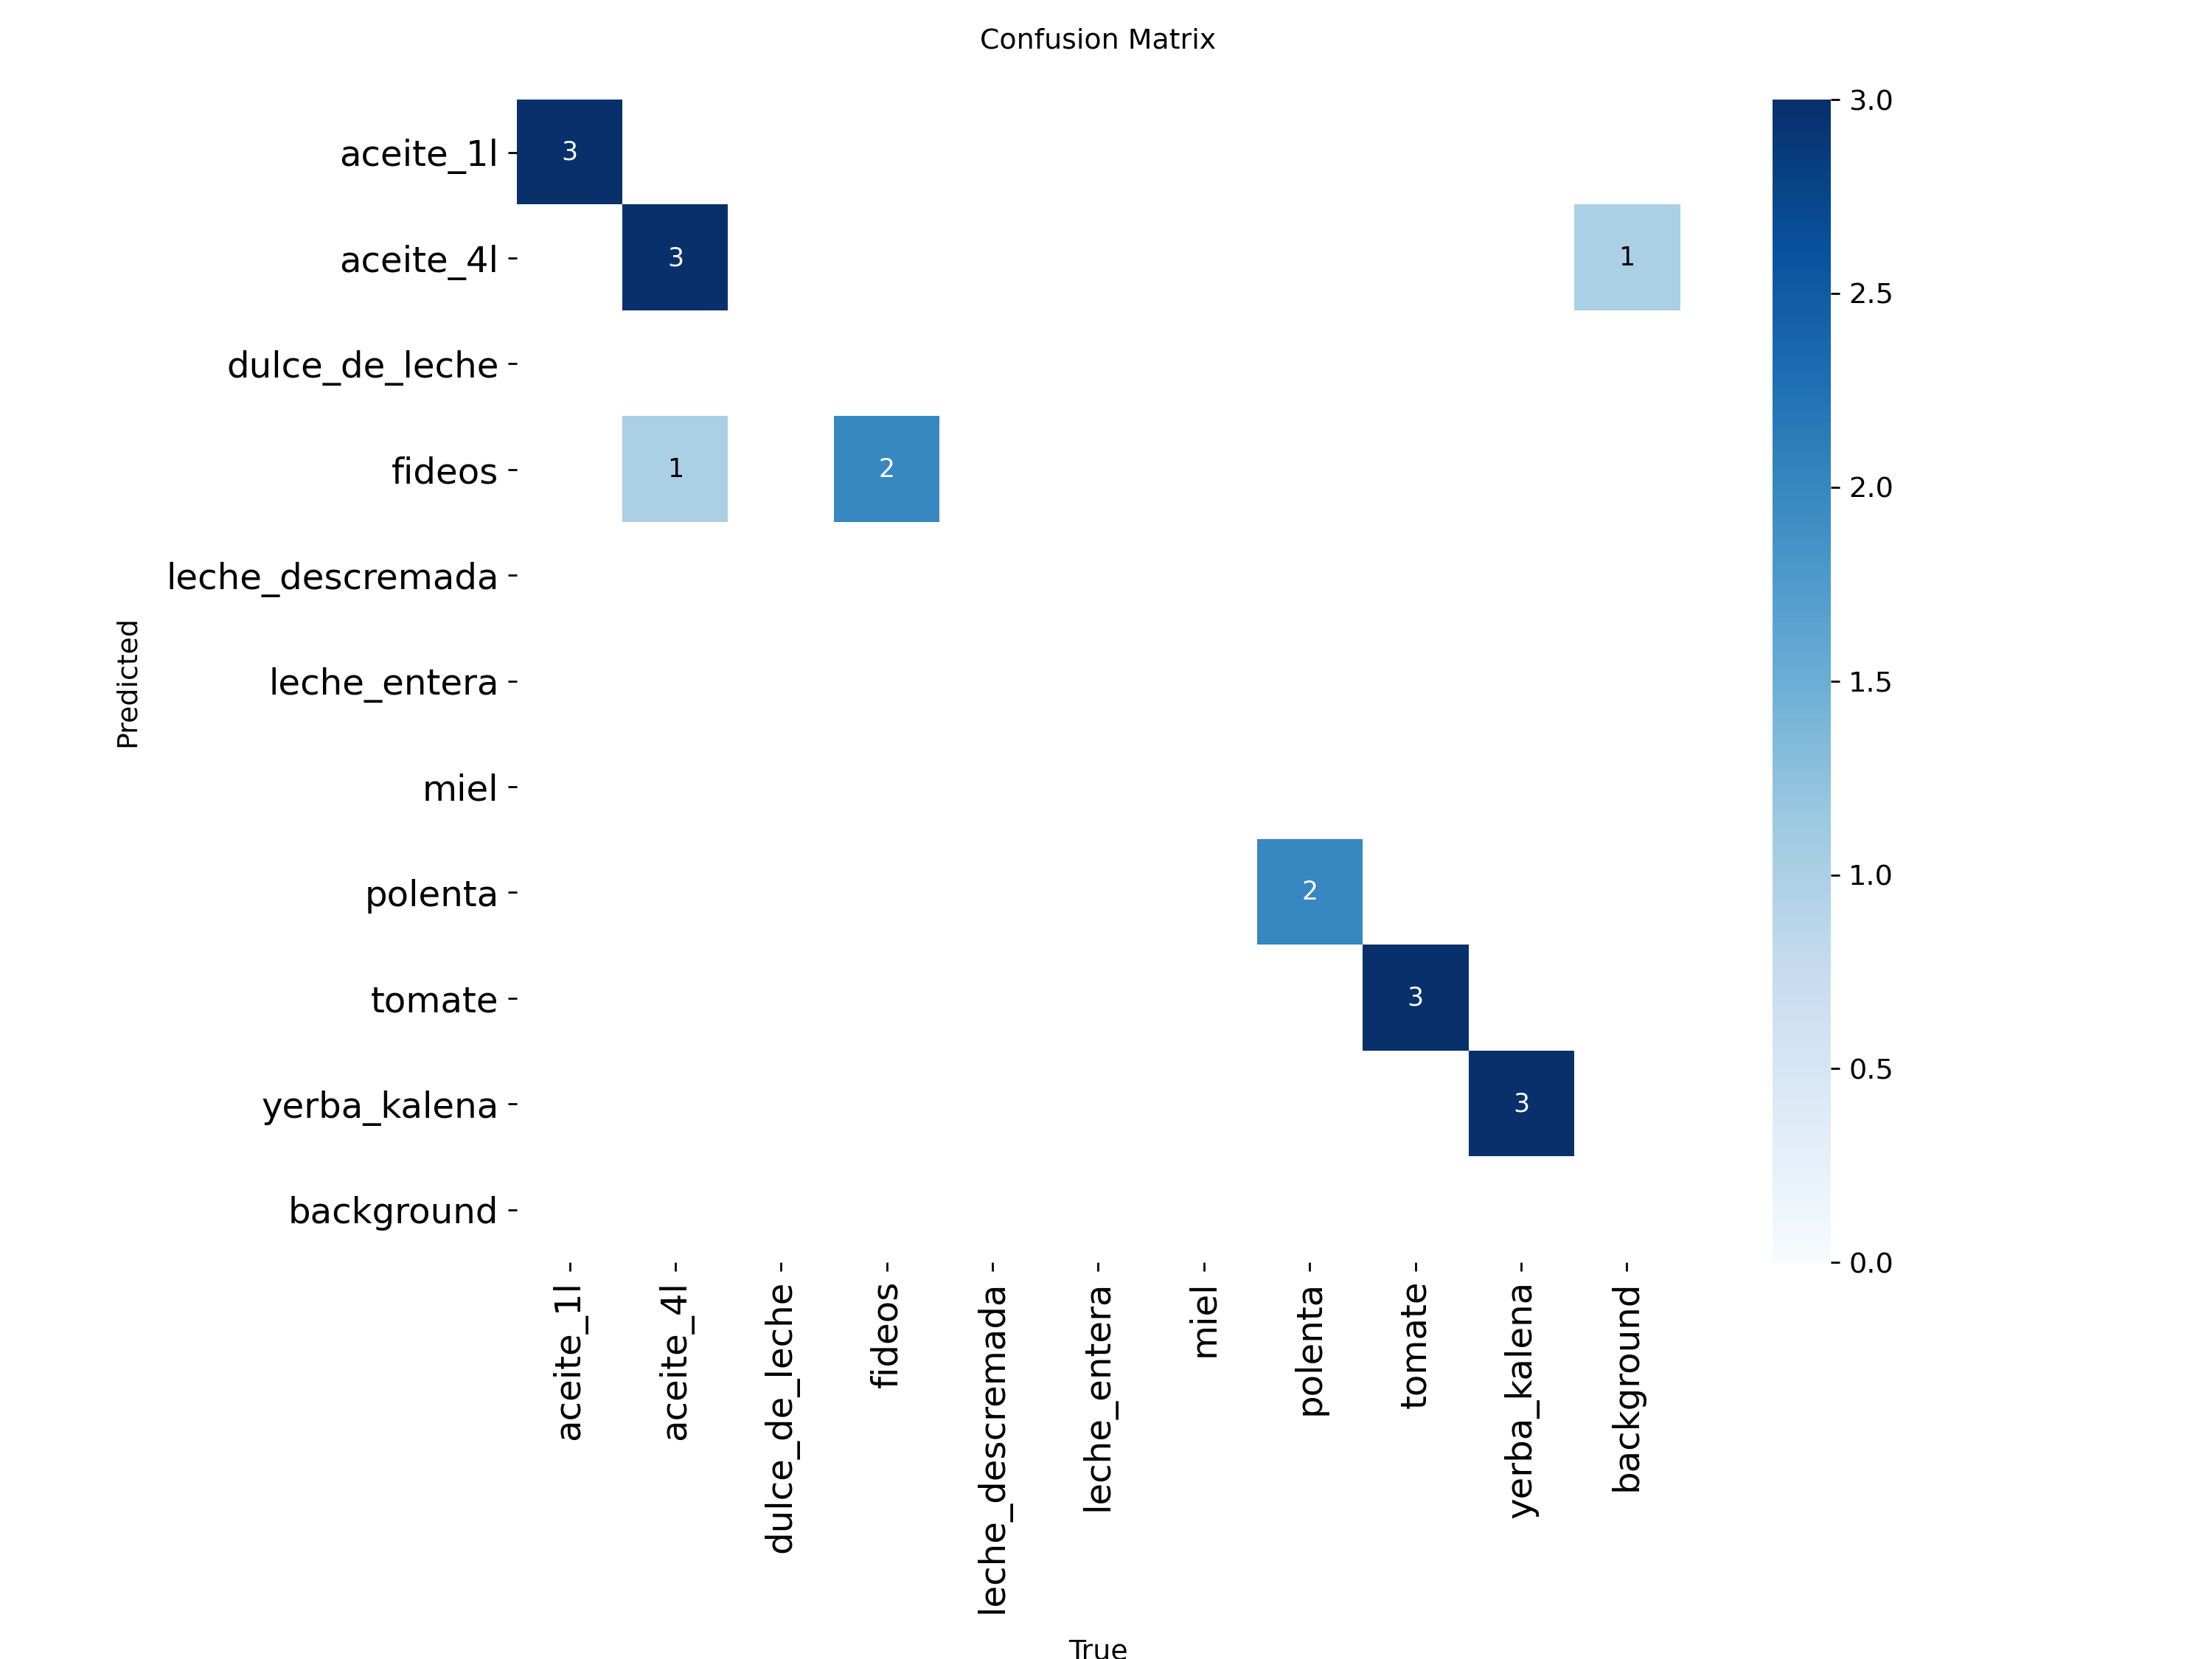
\includegraphics[width=\linewidth]{confusion_matrix_val.png}\\
      \small Matriz de confusión --- validación
    \end{column}
    \begin{column}{0.48\textwidth}
      \centering
      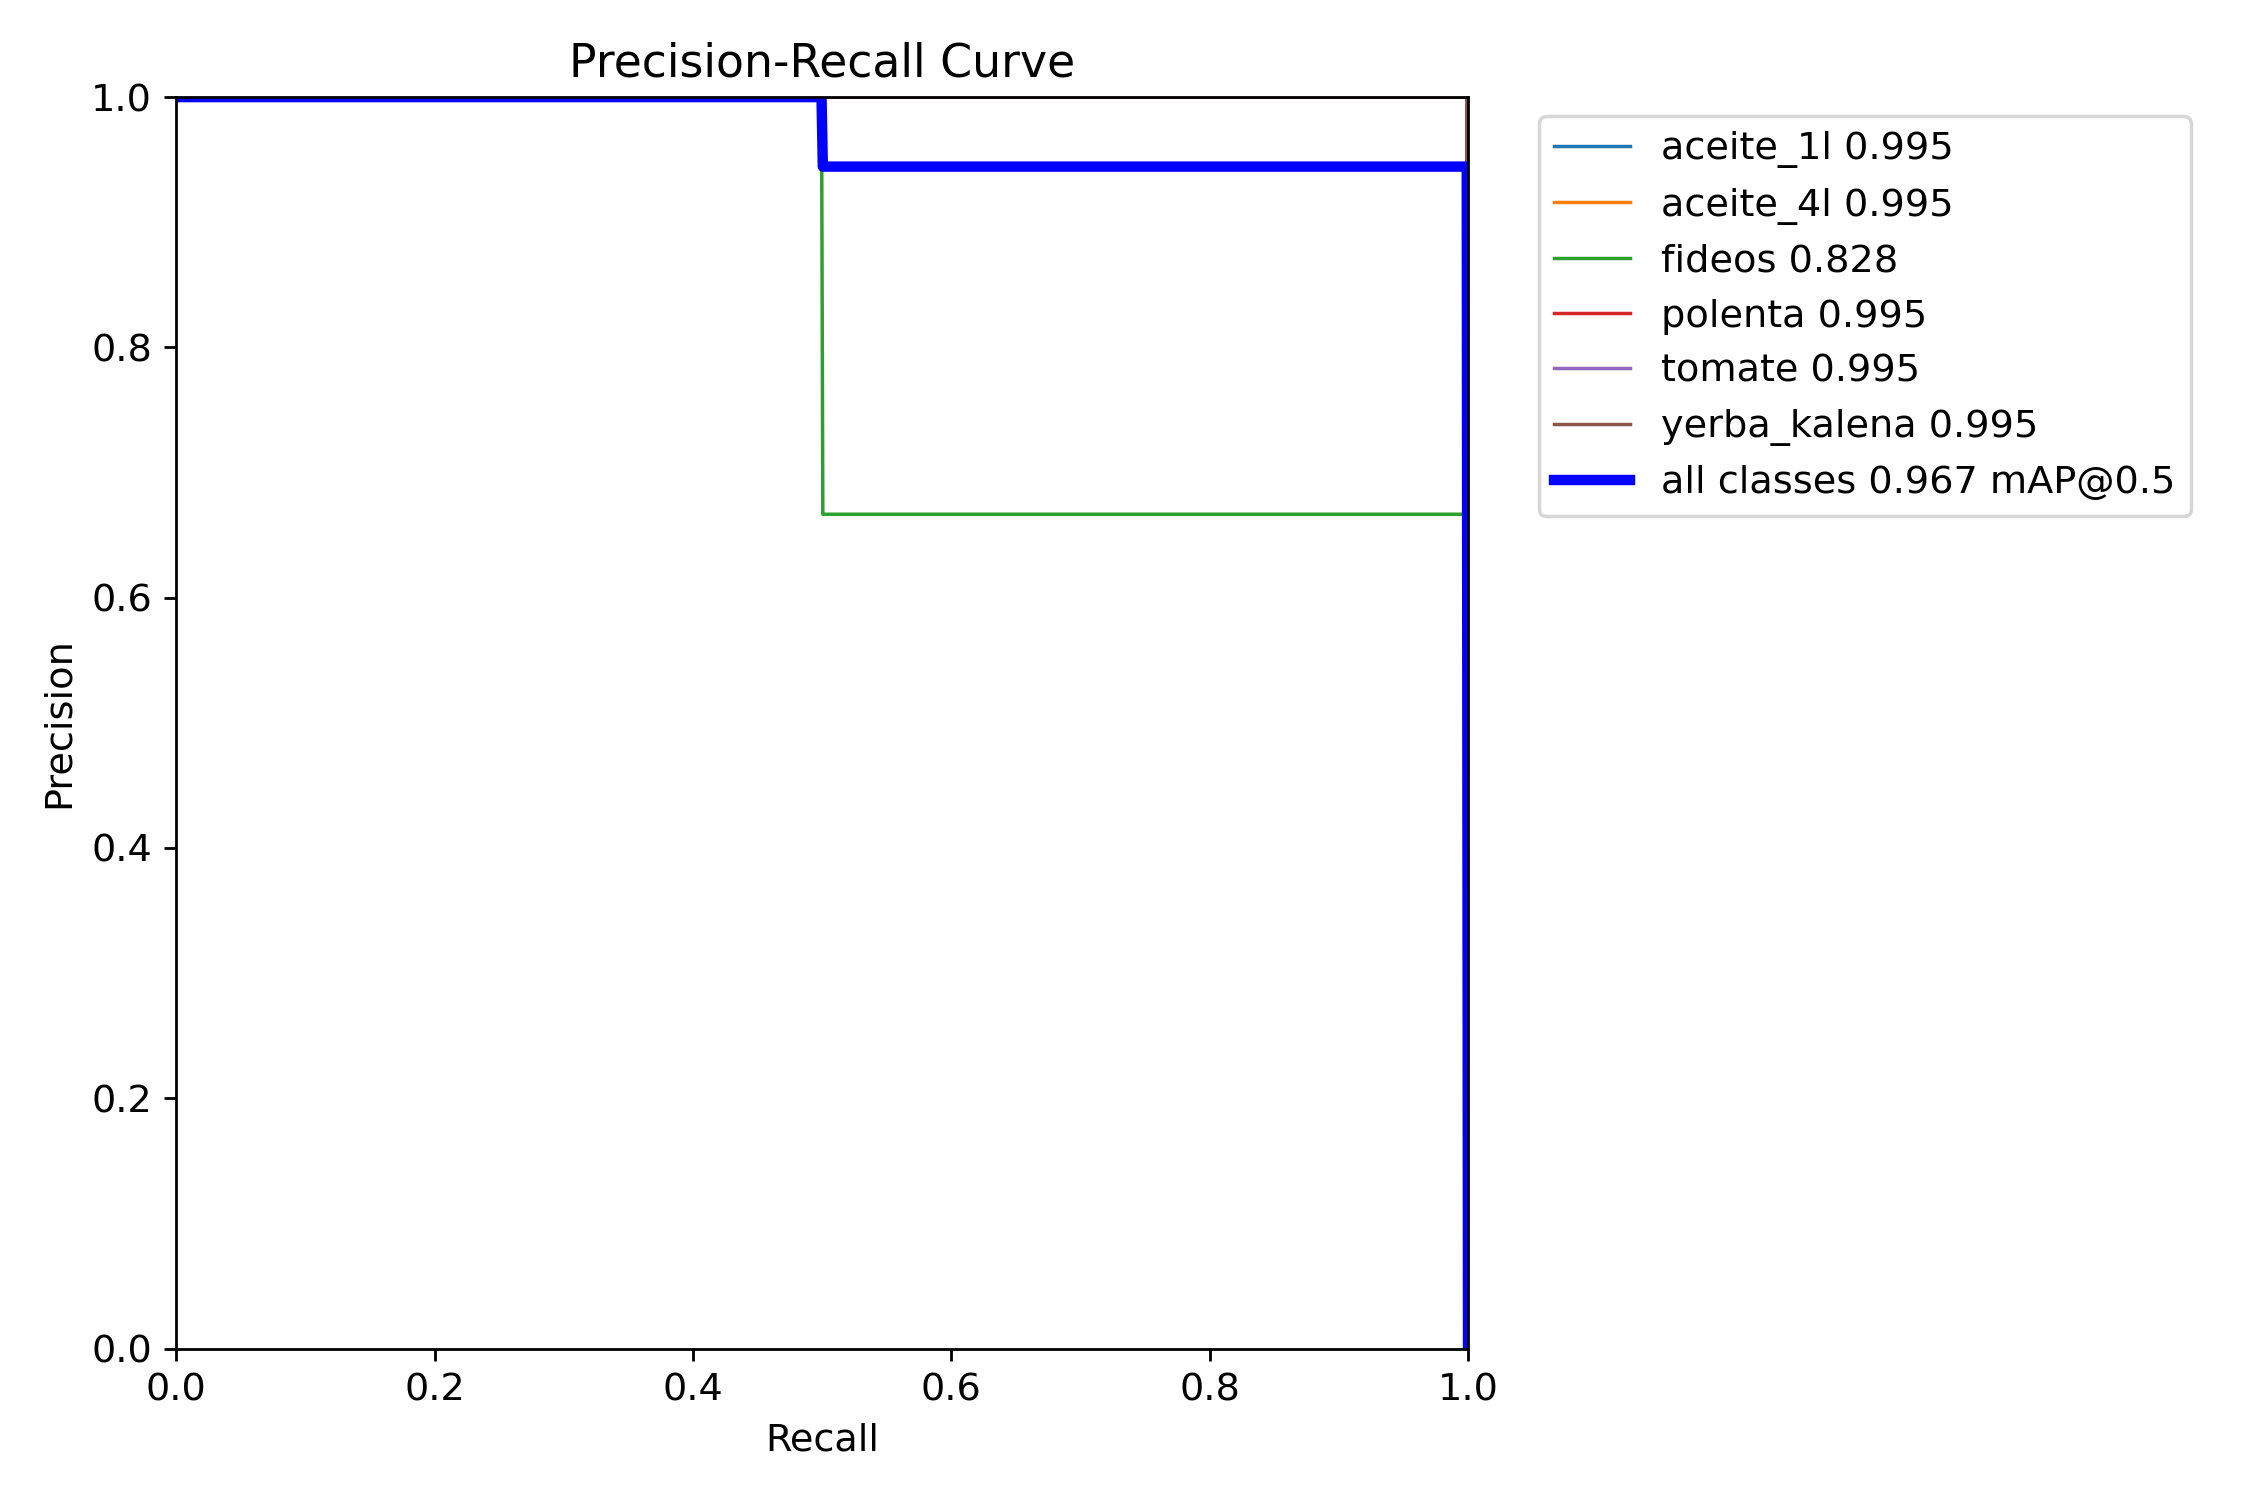
\includegraphics[width=\linewidth]{BoxPR_curve_val.png}\\
      \small Curvas Precision-Recall --- mAP@0.5 = \textbf{0.967}
    \end{column}
  \end{columns}
  \vspace{0.3cm}
  \centering
  Clases como \textit{aceite\_1l}, \textit{polenta} y \textit{tomate}: precisión perfecta.\\
  Clase problemática: \textit{fideos} (mAP@0.5 = 0.828).
\end{frame}

% ============================================================
% SLIDE 9: Resultados — Test
% ============================================================
\begin{frame}{Resultados: Test Split (YOLO11n)}
  \begin{columns}[T]
    \begin{column}{0.35\textwidth}
      \centering
      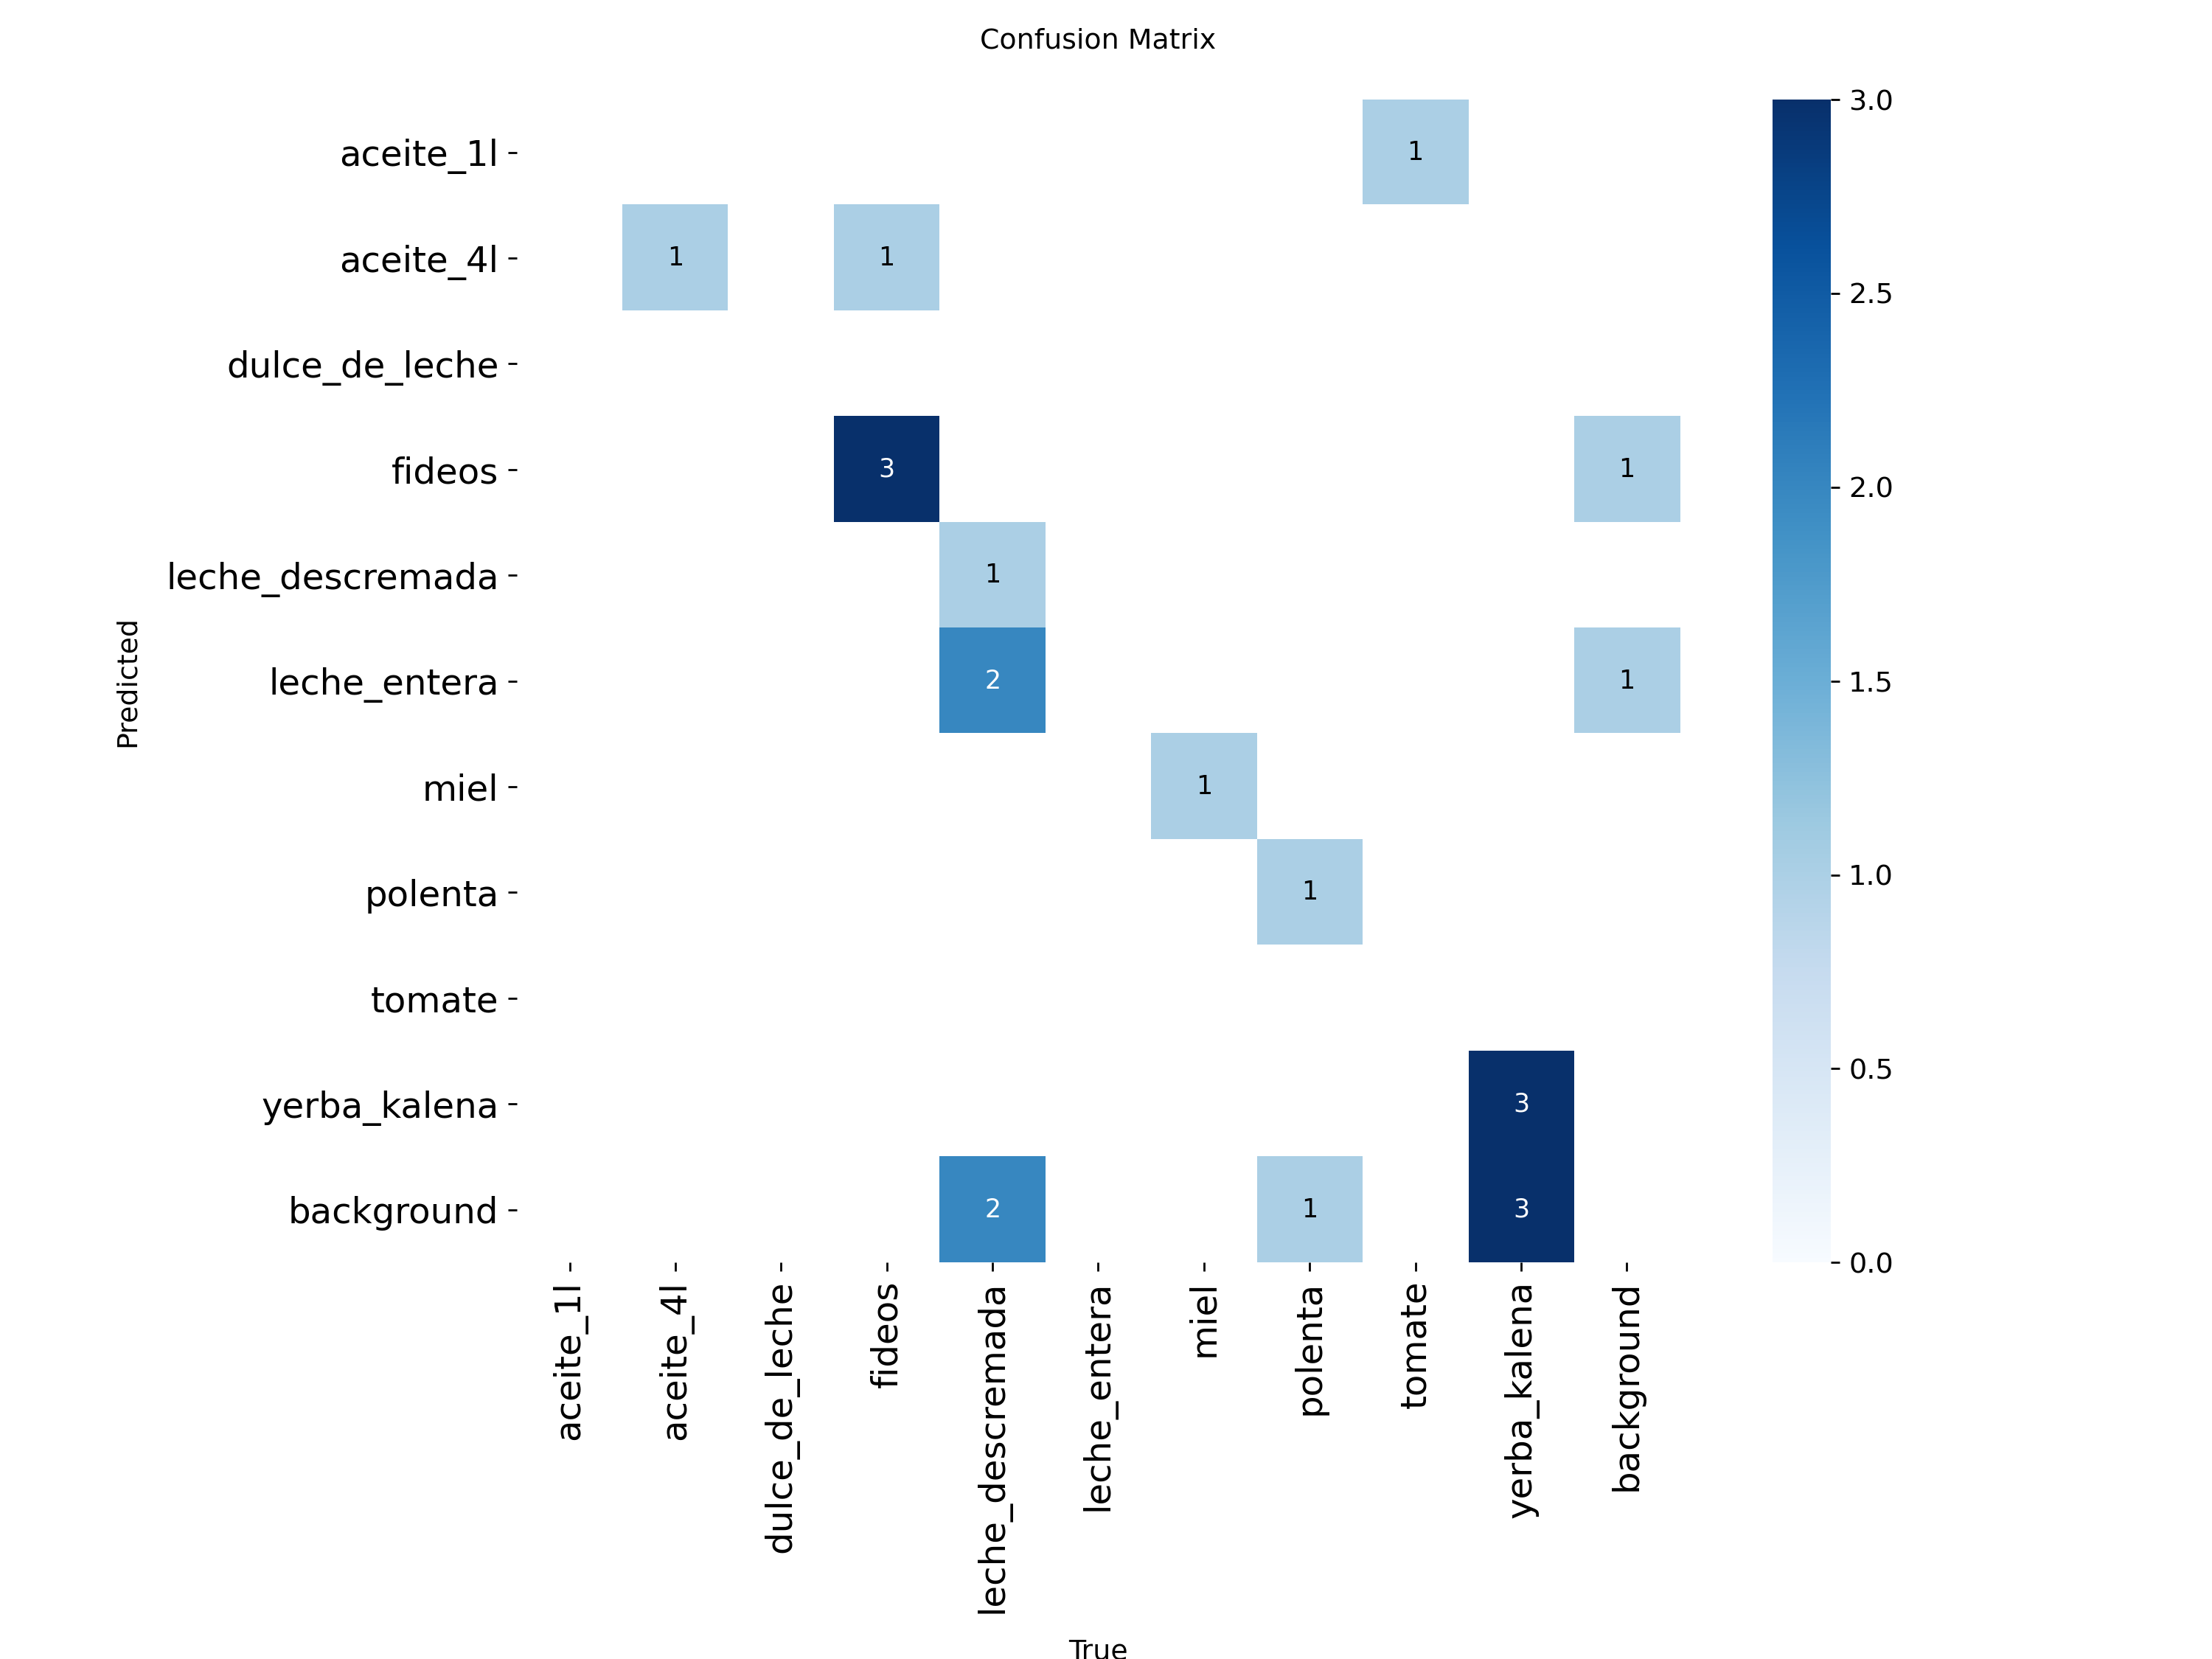
\includegraphics[width=\linewidth]{test_confusion_matrix.png}\\
      {\scriptsize Matriz de confusión --- test}
    \end{column}
    \begin{column}{0.35\textwidth}
      \centering
      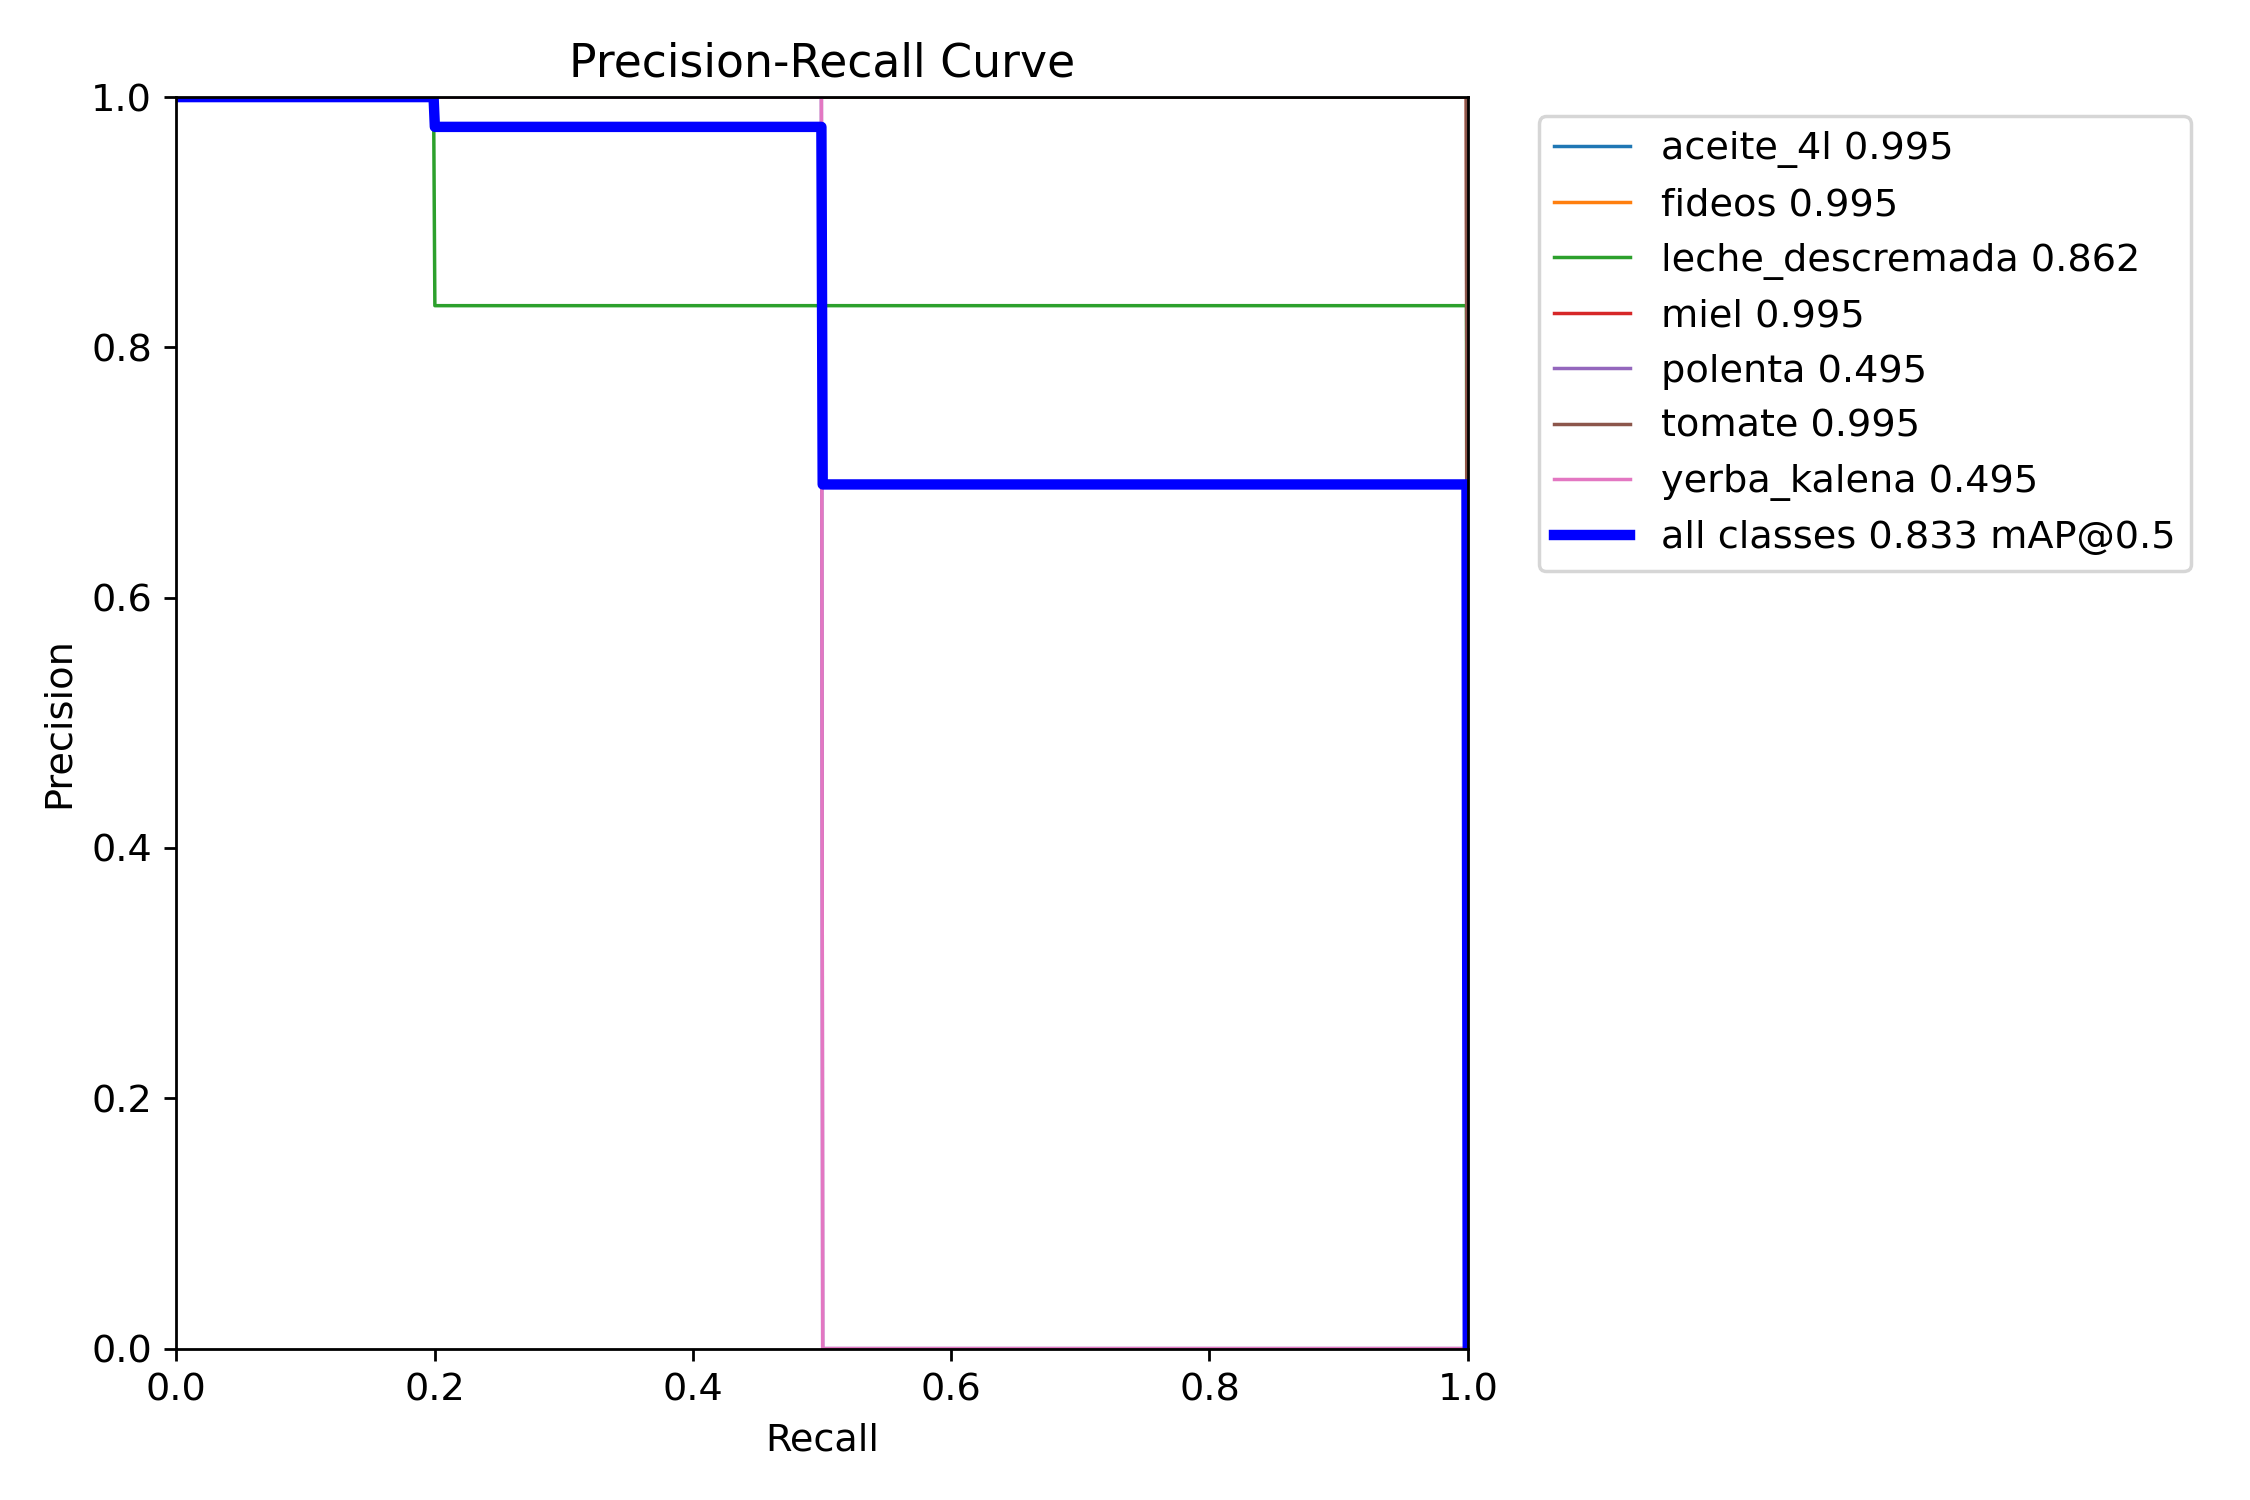
\includegraphics[width=\linewidth]{test_PR_curve.png}\\
      {\scriptsize Curvas PR --- mAP@0.5 = \textbf{0.833}}
    \end{column}
    \begin{column}{0.28\textwidth}
      \small
      \begin{tabular}{lr}
        \toprule
        \textbf{Métrica} & \textbf{Valor} \\
        \midrule
        mAP@0.5     & 0.833 \\
        mAP@0.5:0.95 & 0.755 \\
        Precision    & 0.620 \\
        Recall       & 0.688 \\
        \bottomrule
      \end{tabular}
    \end{column}
  \end{columns}
  \vspace{0.2cm}
  \small
  \textcolor{accentGreen}{\textbf{Perfectas:}} \textit{aceite\_4l, fideos, miel, tomate} (mAP = 0.995) \quad
  \textcolor{accentOrange}{\textbf{Débiles:}} \textit{polenta, yerba\_kalena} (mAP = 0.495)
\end{frame}

% ============================================================
% SLIDE 10: Predicciones cualitativas
% ============================================================
\begin{frame}{Predicciones del Modelo}
  \centering
  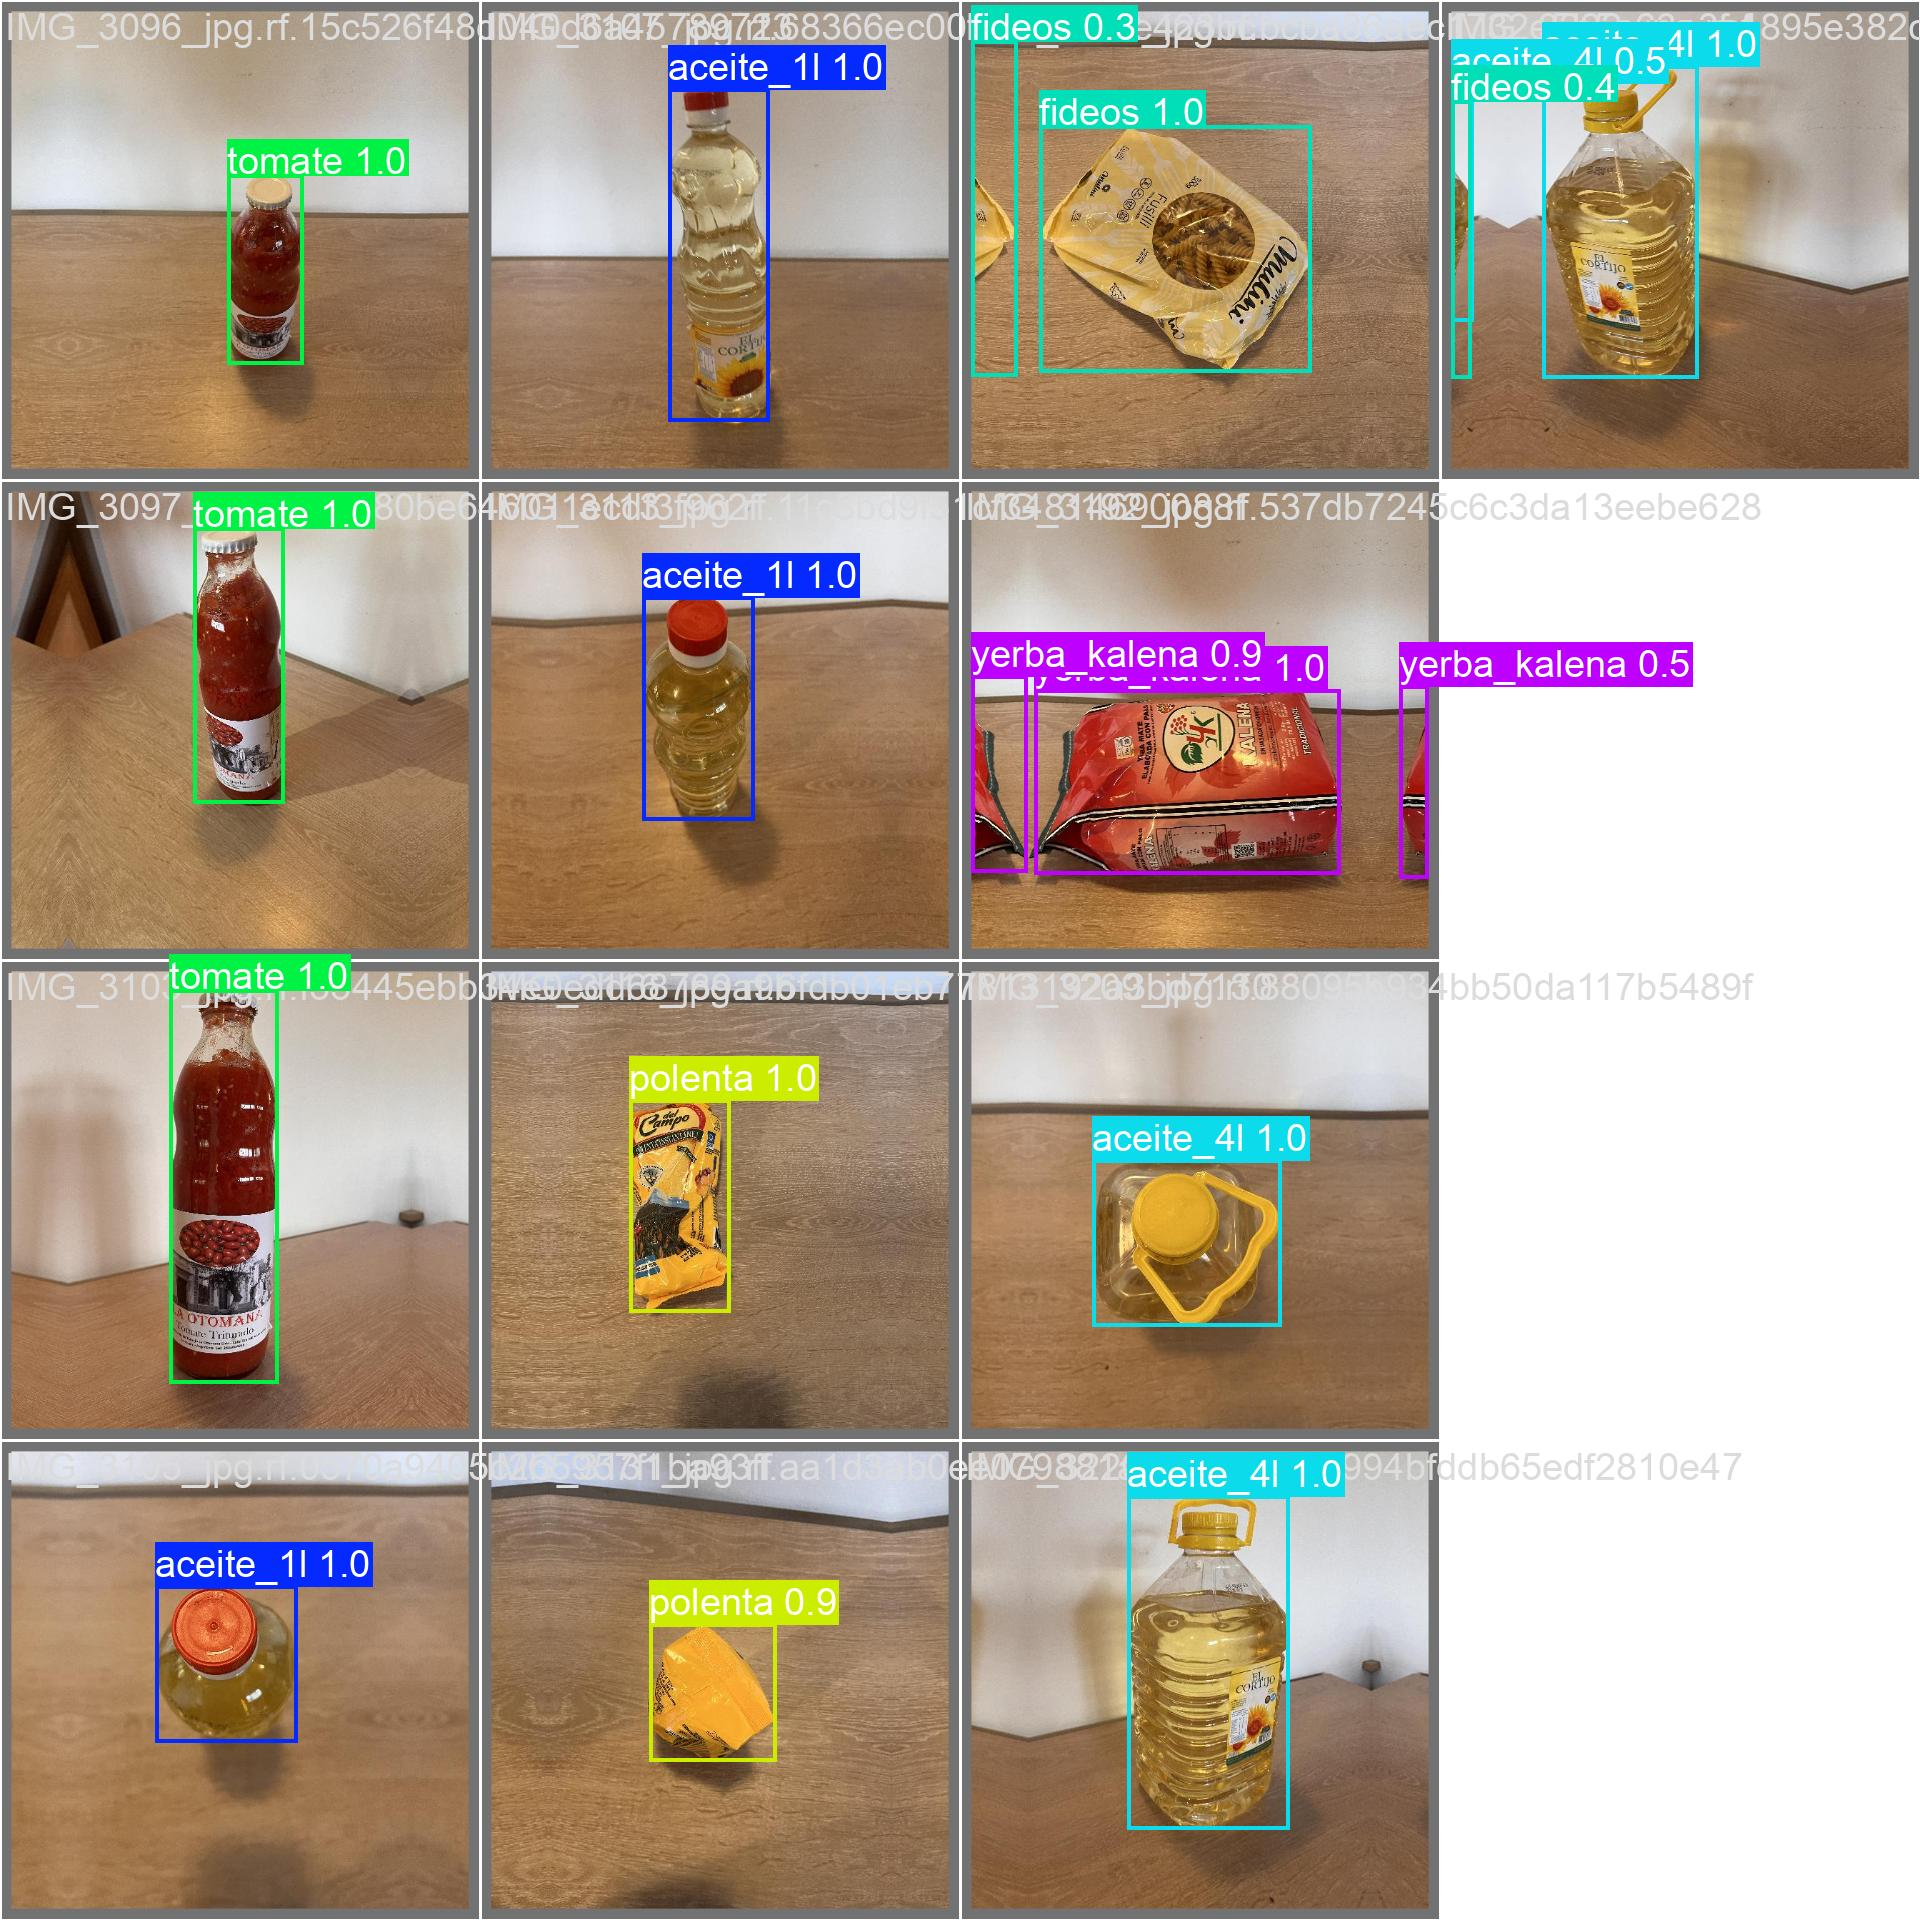
\includegraphics[width=0.75\linewidth, height=0.7\textheight, keepaspectratio]{val_batch0_pred.jpg}\\
  \vspace{0.2cm}
  \small Detecciones con bounding boxes y nivel de confianza generadas por YOLO11n.
\end{frame}

% ============================================================
% SLIDE 11: Demo Video
% ============================================================
\begin{frame}{Demo en Vivo}
  \centering
  \vspace{1cm}
  {\Large \textbf{Video demo}}\\
  \vspace{0.5cm}
  {\large Duración: máx. 2 minutos}\\
  \vspace{1cm}
  \begin{columns}[T]
    \begin{column}{0.45\textwidth}
      \begin{enumerate}
        \item Mesa vacía, sistema corriendo
        \item Agregar productos de a uno
        \item Lista acumulándose en panel lateral
      \end{enumerate}
    \end{column}
    \begin{column}{0.45\textwidth}
      \begin{enumerate}
        \setcounter{enumi}{3}
        \item Productos difíciles (similares)
        \item Estado final de la mesa
        \item JSON de salida generado
      \end{enumerate}
    \end{column}
  \end{columns}
\end{frame}

% ============================================================
% SLIDE 12: Conclusiones y Trabajo Futuro
% ============================================================
\begin{frame}{Conclusiones}
  \begin{enumerate}
    \item Sistema de autocobro funcional basado \textbf{exclusivamente en CV}, costo \textbf{140--190 USD}
    \item YOLO11n alcanza \textbf{mAP@0.5 = 0.967} en validación, \textbf{0.833} en test
    \item Inferencia en tiempo real: $>$15 FPS en laptop, $\sim$10 FPS en Raspberry Pi 5
    \item Data augmentation \textbf{crítico}: sin él, mAP cae de 0.833 a 0.512
    \item Lógica multi-frame elimina falsos positivos sin tracker complejo
  \end{enumerate}
  \vspace{0.3cm}
  \begin{block}{Trabajo Futuro}
    \begin{itemize}
      \item Escalar a $\sim$60 clases del catálogo completo
      \item Deploy en Raspberry Pi 5 en condiciones reales
      \item Métricas end-to-end (order-level accuracy)
      \item Integración con sistema de gestión de la mutual
    \end{itemize}
  \end{block}
\end{frame}

% ============================================================
% SLIDE 13: Cierre
% ============================================================
\begin{frame}{}
  \centering
  \vspace{1.5cm}
  {\Large \textbf{¡Gracias!}}\\
  \vspace{0.5cm}
  {\large ¿Preguntas?}\\
  \vspace{1cm}
  \small
  \textbf{Repositorio:} github.com/BelCattaneo/vpc2\_autocobro\\
  \vspace{0.3cm}
  Cattaneo $\cdot$ Ciarrapico $\cdot$ Pryszczuk\\
  Grupo 4 --- CEIA FIUBA --- 2026
\end{frame}

\end{document}
